\documentclass [a4paper,10pt]{article}
\newcommand{\n}[1]{\textbf{#1}}
\newcommand{\e}[1]{\textcolor{red}{#1}}
\linespread {1.5}
\usepackage[brazilian]{babel}
\usepackage[utf8]{inputenc}
\usepackage[T1]{fontenc}
\usepackage{amsfonts}
\usepackage{amsmath}
\usepackage{amssymb}
\usepackage{amsthm}
    \newtheorem{de}{Definicao}
    \newtheorem{te}{Teorema}
    \newtheorem{pa}{Prova}
    \newtheorem{cl}{Corolário}
    \newtheorem{pr}{Proposição}
\usepackage[ruled,vlined]{algorithm2e}
\usepackage{caption}
\usepackage{subcaption}
\usepackage{booktabs}
\usepackage{multirow}
\usepackage{fancyhdr}
\usepackage{verbatim}
\usepackage{alltt}
\usepackage{fancyvrb}
\usepackage{graphicx,xcolor}
\usepackage{listings}
\lstset{numbers=left,
stepnumber=1,
firstnumber=1,
numberstyle=\tiny,
extendedchars=false,
breaklines=flase,
tabsize=2,
showtabs=true,
tab=\textcolor{gray}{$\cdots$},
keywordstyle=\color{blue},
frame=tb,
basicstyle=\footnotesize,
stringstyle=\ttfamily,
showstringspaces=false}
\renewcommand{\lstlistingname}{Programa}
\renewcommand{\lstlistlistingname}{Lista de Listagens}
\usepackage[pdftex]{hyperref}
\hypersetup{colorlinks,%
linkcolor=red}

\begin{document}

\noindent\rule{\textwidth}{2pt}\\[-3mm]
    \linespread {0.7} {
    \begin{Verbatim}[fontsize=\small]
__/\\\\\\\\\\\\\\\__/\\\\\\\\\\\\\________________/\\\\\\\\\_____        
 _\/\\\///////////__\/\\\/////////\\\____________/\\\///////\\\___       
  _\/\\\_____________\/\\\_______\/\\\___________\///______\//\\\__      
   _\/\\\\\\\\\\\_____\/\\\\\\\\\\\\\/______________________/\\\/___     
    _\/\\\///////______\/\\\/////////_____________________/\\\//_____    
     _\/\\\_____________\/\\\___________________________/\\\//________   
      _\/\\\_____________\/\\\_________________________/\\\/___________  
       _\/\\\\\\\\\\\\\\\_\/\\\________________________/\\\\\\\\\\\\\\\_ 
        _\///////////////__\///________________________\///////////////__
    \end{Verbatim}
    \begin{alltt}
        \hspace{1cm} Métodos Numéricos em ALgebra Linear (MAC0300)
    \end{alltt}
    \vspace{-3mm}
    \rule{\textwidth}{2pt}\\[-6mm]

    \begin{center}
        \n{Por}\\[-0.5mm]
        $\quad${\small Caio Vinícius Dadauto$\quad$7994808}\\[-2mm]
        {\tiny \n{02/11/2014}}\\[4mm]
    \end{center}

    \vspace{2cm}

    As implementações deste trabalho foram executadas em uma máquina com as seguites configurações:\\
    {\linespread{1}
        \begin{tabular}{l r}    
            \hspace{2.5cm}\n{\small OS}      & \small Arch Linux\\
            \hspace{2.5cm}\n{\small Kernel}  & \small x86\_64 Linux 4.1.5-1-ARCH\\
            \hspace{2.5cm}\n{\small CPU}     & \small Intel Core i5-4200 CPU @ 2.6GHz\\
            \hspace{2.5cm}\n{\small RAM}     & \small 3862MiB
        \end{tabular}
    }

    \section{Gradientes Conjugados}
    Gradientes conjugados é um método iterativo para resolução de problemas lineares,
    $$
    Ax = b\quad A \in \mathbb{R}^{n\mathrm{x}n}\;\;x,b \in \mathbb{R}^n
    $$
    onde $A$ é simétrica e positiva definida. Este método é, normalmente, utilizado para resolver sistemas lineares
    que possuem dimensão grande o suficiente para tornar os métodos diretos impraticáveis devido a sua complexidade
    de $\mathcal{O}(n^3)$.
    
    \begin{de}
        Seja a matriz A simétrica. Dois vetores $a$ e $b$ são ditos A-ortogonal se,
            $$
                <a, b>_A := <Aa, b> = <a, A^Tb> = a^TAb = 0
            $$
    \end{de}

    \begin{pr}
        Seja A positiva definida e um conjunto ${d_0, ..., d_n}$ de $n$ vetores não nulos A-ortogonal, ou seja,
        $<d_i, d_j>_A = 0$ para $i \neq j \in {0, ..., n}$.  Então este conjunto é linearmente independente.
    \end{pr}
    \begin{pa}
        Seja um conjunto de coeficientes $\alpha_i$, tais que:
        $$
            \alpha_0d_0 + \cdot\cdot\cdot + \alpha_nd_n = 0
        $$
        então, multiplicando por $A$ e $d_i^T$ qualquer, tem-se que:
        $$
            \alpha_id_i^TAd_i = 0
        $$
        pois, o conjunto dos vetores $d$'s é A-ortogonal. Como $A$ é definida positiva, então $d_i^TAd_i$ > 0.
        Assim, $\alpha_i = 0$ para qualquer $i$, ou seja, o conjunto dos vetores A-ortogonal é linearmente independente.

        \hfill$\blacksquare$
    \end{pa}

    Dessa forma, voltando ao problema do sistema linear $Ax = b$, seja um conjunto $\mathcal{B} = [d_0, ..., d_{n -1}]$
    A-ortogonal e $x^*$ a solução de $Ax = b$, temos que:
    $$
    x^* = \alpha_0d_0 + \cdot\cdot\cdot + \alpha_{n - 1}d_{n - 1}
    $$
    pois $\mathcal{B}$ gera $\mathbb{R}^n$. Multiplicando por $A$ e $d_i^T$ qualquer, temos que:
    $$
    \alpha_i = \frac{d_i^TAx^*}{d_i^TAd_i} = \frac{d_i^Tb}{d_i^TAd_i} = \frac{<d_i, b>}{<d_i, d_i>_A}
    $$
    dessa forma, tem-se ainda que:
    \begin{equation}\label{eq:solucao}
        x^* = \sum_{i = 0}^{n - 1}\frac{<d_i, b>}{<d_i, d_i>_A}d_i
    \end{equation}

    Como o método dos gradientes conjugados é um método iterativo, é possível inferir que podemos gerar novos valores
    de $x$ a partir das direções em $\mathcal{B}$, ou seja, suponha-se que:
    $$
    x_{k+1} = x_k + \alpha_k d_k
    $$
    essa inferência traz a tona o sentido iterativo do método. Porém, ainda devemos determinar como $\alpha_k$ deve se comportar.
    A partir da igualdade \eqref{eq:solucao} é possível supor que $\alpha_k$ se comporte da seguinte maneira,
    $$
    \alpha_k = \frac{<b - Ax_k, d_k>}{<d_k, d_k>_A} = -\frac{<Ax_k - b, d_k>}{<d_k, d_k>_A}
    $$
    Pois, se considerarmos que $||e_k|| := ||x^* - x_k|| \geq ||x^* - x_{k + 1}|| := ||e_{k + 1}||$ e que $x^* = x_n$, então
    $$
    x^* = x_0 + \sum_{i = 0}^{n - 1}\frac{<Ax_i - b, b>}{<d_i, d_i>_A}d_i
    $$
    já que $\alpha_n$ deve ser nulo. E ainda, essa igualdade é equivalente a \eqref{eq:solucao}, devido a $\mathcal{B}$
    ser uma base.

    É importante notar que o método dos gradientes conjugados é equivalente ao problema,
    $$
    \mathrm{min}\;\;f(x) = \frac{1}{2}x^TAx - b^Tx
    $$
    pois, como essa fução é convexa, basta verificar a condição de otimalidade de primeira ordem, ou seja, $\nabla f = 0$
    para determinar o ponto de mínimo de $f(x)$. O que é justamente resolver o problema $Ax = b$, já que $\nabla f = Ax - b$.
    Portanto, desta última observação, denotamos $g_k = Ax_k - b$, onde $g$ é o gradiente de $f$, e então:
    $$
    x^* = x_0 - \sum_{i = 0}^{n - 1}\frac{<g_i, b>}{<d_i, d_i>_A}d_i
    $$

    \begin{te}
        Seja $\mathcal{B}$ um conjunto de $n$ vetores A-ortogonal. Para qualquer $x_0$ a sequência ${x_k}$ gerada por
        $$
        x_{k+1} = x_k + \alpha_k d_k
        $$
        com
        $$
        \alpha_k = -\frac{<g_k, d_k>}{<d_k, d_k>_A};\quad g_k = Ax_k - b
        $$
        converge para a única solução de $Ax = b$, $x^* = x_n$.
    \end{te}
    \begin{pa}
        Da recorrência de $x_k$ e do fato de que $x^* = x_n$, temos que:
        $$
        x^* - x_0 = \alpha_0d_0 + \cdot\cdot\cdot + \alpha_{n - 1}d_{n - 1}
        $$
        como sempre, multiplicando por A e fazendo o produto escalar por $d_k$ qualquer, temos:
        $$
        \alpha_k = \frac{<d_k, x^* - x_0>_A}{<d_k, d_k>_A}
        $$
        Dessa forma, basta provar que $\alpha_k$ é da forma $-\frac{<g_k, d_k>}{<d_k, d_k>_A}$.

        Para isso tomemos a seguinte igualdade para $x_k$ qualquer:
        $$
        x_k - x_0 = \alpha_0d_0 + \cdot\cdot\cdot + \alpha_{k - 1}d_{k - 1}
        $$
        de forma análoga, porém fazendo o produto escalar por $d_k$, tem-se que:
        $$
        <d_k, x_k - x_0>_A = 0
        $$

        Assim, temos que:
        \begin{eqnarray*}
            \alpha_k & = & \frac{<d_k, (x^* - x_k) + (x_k - x_0)>_A}{<d_k, d_k>_A}\\
             & = & \frac{<d_k, x^* - x_k>_A + <d_k, x_k - x_0>_A}{<d_k, d_k>_A}\\
             & = & \frac{<d_k, x^* - x_k>_A}{<d_k, d_k>_A}\\
             & = & \frac{d_k^T(Ax^* - Ax_k)}{<d_k, d_k>_A}\\
             & = & \frac{d_k^T(b - Ax_k)}{<d_k, d_k>_A}\\
             & = & -\frac{(Ax_k - b)^Td_k}{<d_k, d_k>_A}\\
             & = & -\frac{g_k^Td_k}{<d_k, d_k>_A}\\
             \alpha_k & = & -\frac{<g_k, d_k>}{<d_k, d_k>_A}
        \end{eqnarray*}
        O que demonstra a convergência dados a recorrência e o $\alpha$ apresentados pelo teorema.

        \hfill$\blacksquare$
    \end{pa}

    \subsection{Algoritmo}
    Do último Teorema da seção anterior, podemos inferir o seguinte algoritmo:

    \begin{algorithm}[!hb]
        $x_k = 0$, $g_k = -b$, $d_k = b$\\
        \While{$||g_k|| > \epsilon$}{
            $\alpha_k  = -\frac{<g_k, d_k>}{<d_k, d_k>_A}$\\
            $x_{k}     = x_k + \alpha_k d_k$\\
            $g_{k}     = Ax_{k} - b$\\
            $\beta_k   = \frac{<g_{k}, d_k>_A}{<d_k, d_k>_A}$\\
            $d_{k}     = -g_{k} + \beta_kd_k$
        }
        \caption{\small Algoritmo para  o método dos gradientes conjugados.}
    \end{algorithm}

    Para verificar a corretude desse algoritmo, notemos o seguinte teorema.

    \begin{te}
        O algoritmo é um método de gradientes conjugados, pois as seguintes afirmações são verdadeiras:\\
            \begin{tabular}{l l}    
                \hspace{2.5cm}\n{(i)}   & ${g_0, g_1, ..., g_k} = {g_0, Ag_0, ..., A^kg_0}$\\
                \hspace{2.5cm}\n{(ii)}  & ${d_0, d_1, ..., d_k} = {g_0, Ag_0, ..., A^kg_0}$\\
                \hspace{2.5cm}\n{(iii)} & $d_kAd_i$ para qualquer $i < k$\\
                \hspace{2.5cm}\n{(iv)}  & $\alpha_k = \frac{<g_k, g_k>}{<d_k, d_k>_A}$\\
                \hspace{2.5cm}\n{(v)}   & $\beta_k = \frac{<g_{k + 1}, g_{k + 1}>}{<g_k, g_k>}$
            \end{tabular}
    \end{te}

    Assim, a partir dos itens $(iv)$ e $(v)$ do teorema acima, é possível escrever outro algoritmo para o método dos
    gradientes conjugados com a vantagem deste ser menos custoso que o primeiro, como segue a baixo:

    \begin{algorithm}[!ht]
        $x_k = 0$, $g_k = b$, $d_k = b$\\
        \While{$||g_k|| > \epsilon$}{
            $g_{k - 1} = g_k$\\
            $\alpha_k  = \frac{<g_k, g_k>}{<d_k, d_k>_A}$\\
            $x_{k}     = x_k + \alpha_k d_k$\\
            $g_{k}     = g_k - \alpha_kAd_k$\\
            $\beta_k   = \frac{<g_k, g_k>}{<g_{k - 1}, g_{k - 1}>}$\\
            $d_{k}     = g_{k} + \beta_kd_k$
        }
        \caption{\small Algoritmo para  o método dos gradientes conjugados otimizado.}
    \end{algorithm}

    Apesar da privisão teórica impor que o método atinge $x^*$ após $n$ iterações, isso não é normalmente necessário
    para que o método atinga um valor satisfatório de $x^*$, ou seja, $g_k < \epsilon$, onde $\epsilon$ é da ordem
    da precisão de máquina.

    \section{Implementação}
    Para a implementação do método, buscou-se uma forma mais adequada para o armazenamento da matriz esparsa $A$ (caso
    onde o uso método iterativo faz sentido) de forma que o produto $Ad$ fosse de complexidade $\mathcal{O}(n)$.
    Assim, a matriz esparsa $A$ foi armazena segundo o padrão $Yale$. Esse padrão consiste em armazenar três vetores
    distintos denominados $A$, $IA$ e $JA$. Em $A$ são armazenados os valores não nulos da matriz esparsa e em $JA$ são
    armazenados os indices das colunas onde os respectivos valores não nulos de $A$ se encontram na matriz esparsa. Já
    os indices $i$'s do vetor $IA$ representam os indices das linhas da matriz esparsa, enquanto que cada posição de $IA$
    armazena um indice do vetor $A$, onde esse indice representa o primeiro valor não nulo da linha $i$ na matriz esparsa.
    A leitura da matriz esparsa para o armazenamento no padrão $Yale$ é feita da esquerda para direita de cima para baixo, ou
    seja, ordenada por linha.

    Para testar o algoritmo apresentado na seção anterior, implementou-se um gerador de matrizes esparsas simétricas e definidas
    positivas. Esse gerador foi desenvolvido seguindo o mesmo raciocínio empregado no exemplo da página 300 da referência
    \cite{livro1}, este raciocínio se baseia em criar uma matriz esparsa com diagonal pricipal unitária e com os demais valores fora da diagonal
    inicializados com um valor aleatório segundo uma distribuição uniforme em $[-1, 1]$, mantendo a semetria da matriz. Porém, para
    garantir a caracteristica de esparsidade da matriz $A$, cada valor gerado nessa distribuição uniforme é comparado em móduto com
    um valor $\tau \in (0, 1)$, se o valor gerado pela distribuição for maior que $\tau$, então a entrada na matriz será nula. Além disso, 
    o vetor $b$ do sistema $Ax = b$ é gerado pela mesma distibuição uniforme.

    A implementação segue junto com esse relatório, o arquivo $gerador.c$ contém o gerador de matriz esparsa segundo o que foi
    explicado acima. Já o arquivo $gradienteConjugado.c$ contém a implementação do método explicado na seção anterior, bem como
    um conjunto de função auxiliares para tratar de operações com matrizes e vetores.

    \subsection{Exemplo}
    O exemplo da referência \cite{livro1} é reproduzido a seguir. Foram geradas matriz esparsas para os valores $0.01$,
    $0.05$, $0.1$ e $0.2$ de $\tau$. As dimensões ($n$) das matrizes utilizads neste exemplo foram de $500$ e $1000$.
    Os gráficos a seguir apresentam o resusltado obtido para as 20 primeiras iterações do método.
    \begin{figure}[!ht]
        \centering
        \begin{subfigure}[!hb]{\textwidth}
            \centering
            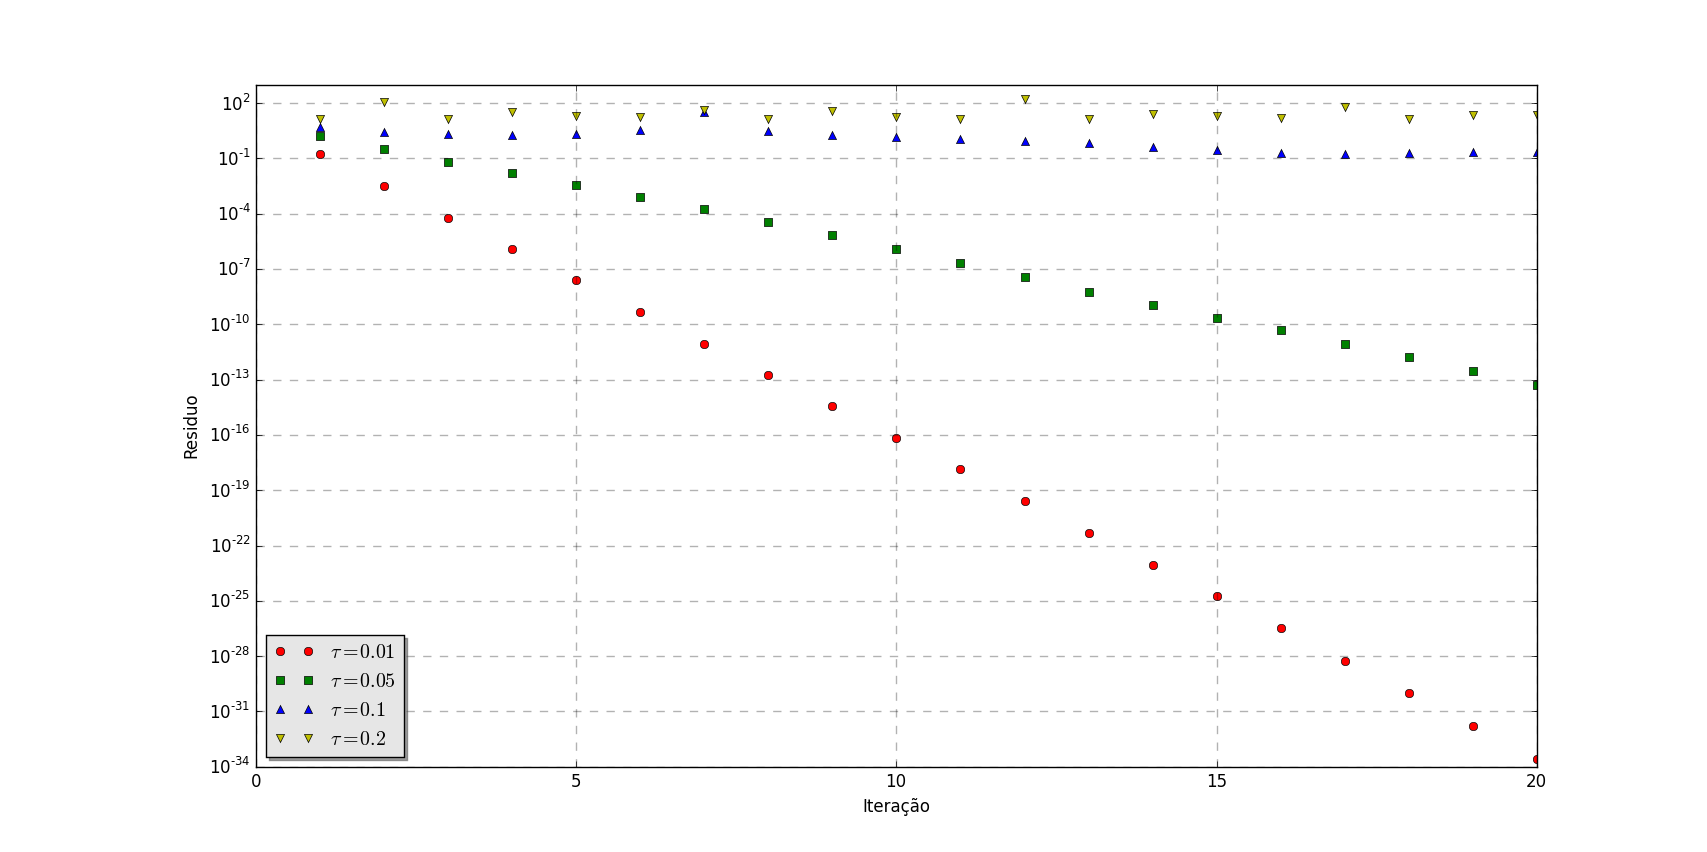
\includegraphics[scale=0.23]{figure_500.png}
            \caption{Matriz de dimensão $n = 500$.}
        \end{subfigure}
        \\
        \begin{subfigure}[!hb]{\textwidth}
            \centering
            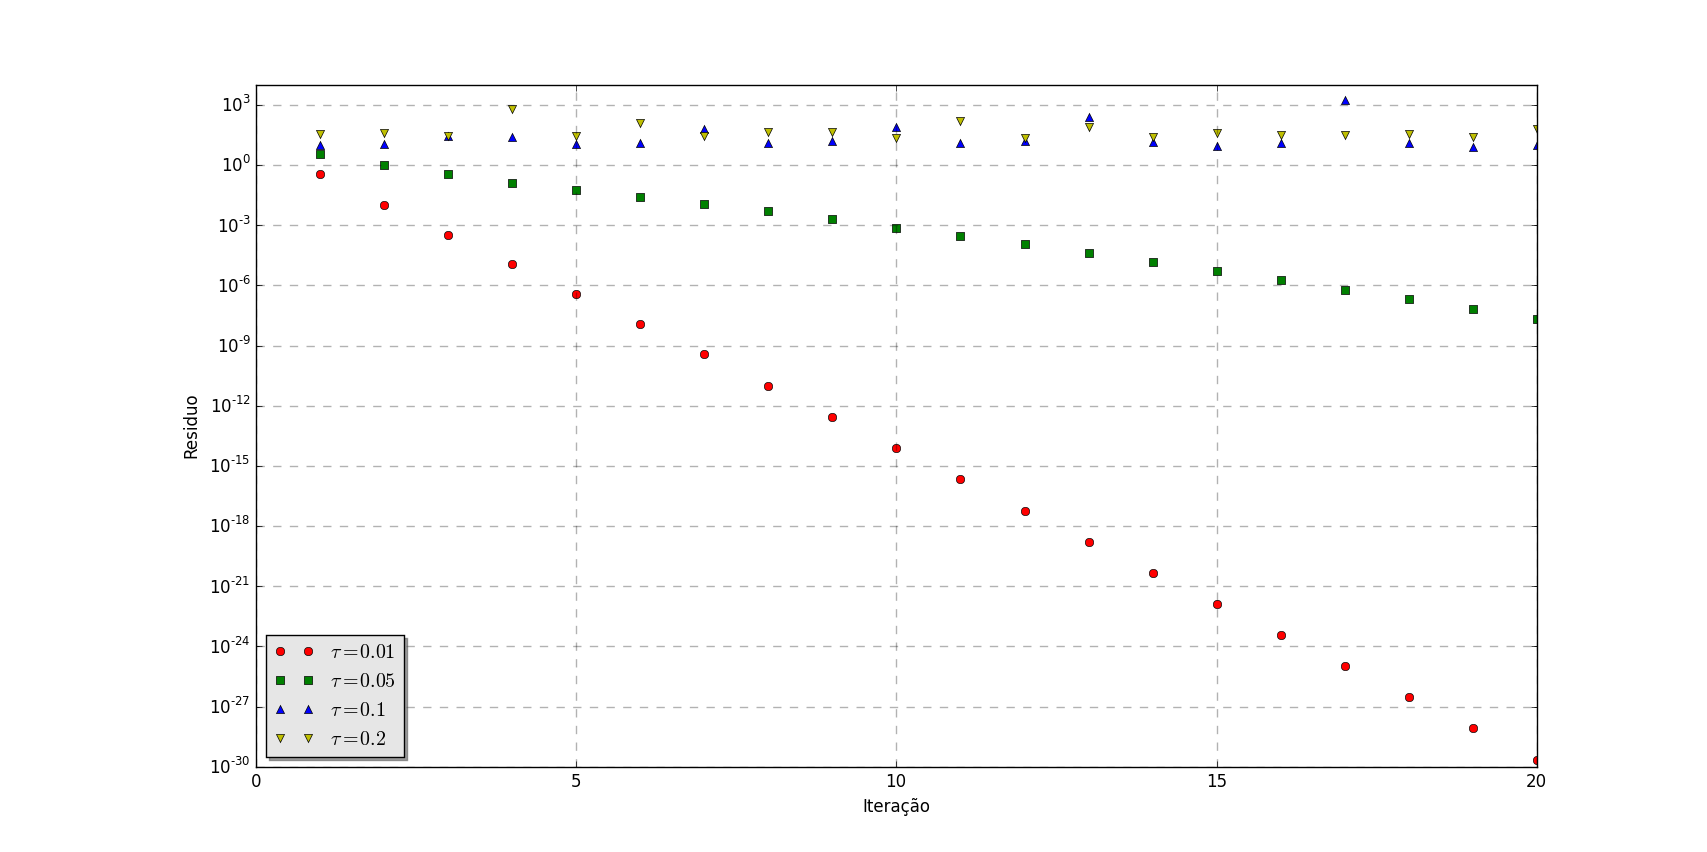
\includegraphics[scale=0.23]{figure_1000.png}
            \caption{Matriz de dimensão $n = 1000$.}
        \end{subfigure}
        \caption{Gráficos para o desenvolvimento do método durante as 20 primeiras iterações
        em função do módulo do resíduo.}
    \end{figure}

    \subsection{Velocidade de Convergência}
    A medição de velociadade é algo complicado de se tratar neste caso, pois a esparcidade da matriz $A$ depênde do
    parâmetro $\tau$ e o condicionamento da matriz $A$ não é garantido, pois os valores da matriz são aleatóriamente
    gerados. Entrento, buscou-se determinar sem muita presição a complexidade do método. Para isso, gerou-se matrizes
    esparsas para $\tau = 0.01$ de dimensões variadas,
    a saber 100, 500, 700, 1000, 1200, 1400, 1600, 2000, 5000, 6000, 8000 e 10000. Não foram tratados
    valoes maiores do que estes pois o método para gerar estas matriz passa a consumir muito tempo de processamento. A cada
    matriz gerado aplicou-se o método dos gradientes conjugados e registou-se o tempo para que o método atingisse um resíduo
    com módulo menor que $10^{-19}$. Assim, plotou-se os pontos gerados do tempo em função da dimensão $n$ e ajustou-se aos pontos
    uma função da forma $y = [0]x^[1]$, obtento um expoente de $1.89$. O que implica em uma complexidade aproximadamente
    $\mathcal{O}(n^2)$. A figura abaixo apresenta o gráfico plotado.
    \begin{figure}[!ht]
        \centering
        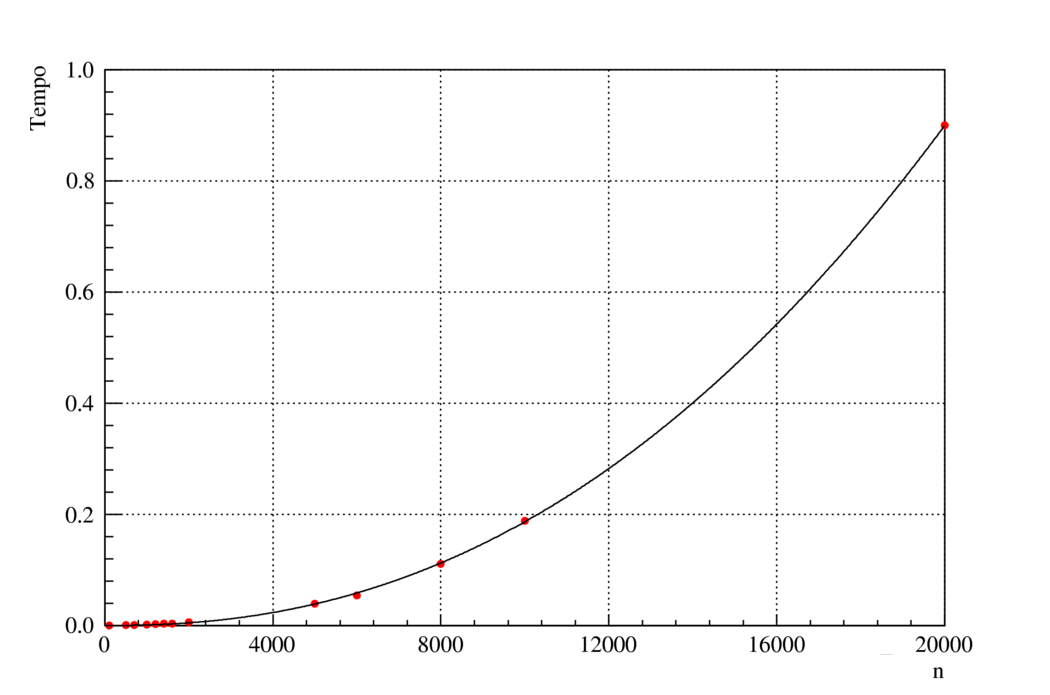
\includegraphics[scale=0.35]{tempo.png}
        \caption{Estimativa da complexiade para o método iterativo.}
    \end{figure}


  \begin{thebibliography}{99}
      \bibitem{livro1} \emph{Lloyd N. Trefethen, David Bau,} Numerical Linear Algebra, Society for Industrial and Applied
Mathematics, Philadelphia, 1997.
      \bibitem{livro2} \emph{Luenberger D.G., Ye Y.,} Linear and nonlinear programming-Springer, 2008.
  \end{thebibliography}
    
\end{document}
    
